\documentclass[a4j,11pt]{ujarticle}
\usepackage{fancyhdr}
%\usepackage{here}
\usepackage[dvipdfmx]{graphicx}
\usepackage{float}
\usepackage{listings}
\usepackage[dvipdfmx]{xcolor}
\renewcommand{\thepage}{\small -- \arabic{page} --}
%\headrulewidth=0pt

% コードブロックの設定
\lstset{
  basicstyle=\ttfamily\small,
  keywordstyle=\color{blue},
  commentstyle=\color{green!50!black},
  stringstyle=\color{red},
  breaklines=true,
  frame=single,
  numbers=left,
  numberstyle=\tiny\color{gray}
}

\rhead{}
\lhead{}
\textheight 234mm
%
\usepackage{amsmath}	% required for `\cases' (yatex added)
\usepackage{bm}
\usepackage{ascmac}	% required for `\screen' (yatex added)

\newcommand{\thisyear}{2025}

\pagestyle{fancy}
\lhead{{\thisyear}年度 プログラミングIII}

\title{{\thisyear}年度 プログラミングIII 第13回 レポート}
\date{\number\year 年\number\month 月\number\day 日}

\author{学籍番号36714137 \\ 山本賢人}
%
%
\begin{document}
%
\maketitle
\clearpage
%
%
\section{はじめに}
%
本レポートでは課題のプログラムの中身と実行結果について報告する。
%
%
\section{演習課題}
\subsection{演習13-1}

与えられたスタックのプログラムを関数やヘッダーごとに分割し、Makefileを作成してコンパイルが行えるようにする。
また、スタックにプッシュされた全要素を表示する機能を追加する。

まず、プログラムの分割から行う。main関数をmain13.cに配置し、ヘッダファイルをincludeする形で実装する。
\begin{lstlisting}[language=C, caption=main13.cの実装]
#include <stdio.h>
#include "task13.h"

int main(void) {
    Stack stk;

    if (StackAlloc(&stk, 100) == -1) {
        printf("スタックの作成に失敗しました\n");
        return 1;
    }

    while (1) {
        int m, x;
        printf("現在のデータ数: %d / %d\n", StackNo(&stk), StackSize(&stk));
        printf("(1)プッシュ (2)ポップ (3)表示 (0)終了: ");
        scanf("%d", &m);
        if (m == 0) {
            break;
        }

        switch (m) {
            case 1:
                printf("データ: ");
                scanf("%d", &x);
                if (StackPush(&stk, x) == -1) {
                    printf("プッシュに失敗しました\n");
                }
                break;
            case 2:
                if (StackPop(&stk, &x) == -1) {
                    printf("ポップに失敗しました\n");
                }
                break;
            case 3:
                printf("スタックの中身: ");
                for (int i = 0; i < StackNo(&stk); i++) {
                    printf("%d ", stk.stk[i]);
                }
                printf("\n");
                break;
            default:
                break;
        }
    }

    StackFree(&stk);

    return 0;
}
\end{lstlisting}

case 3の部分がスタック全表示の新規実装部分である。StackNo関数で現在のスタックポインタ位置を取得し、その数だけループを回して全要素を表示している。

次に、ヘッダファイルの実装を行う。Stack構造体の定義と関数のプロトタイプ宣言を記述する。
\begin{lstlisting}[language=C, caption=task13.hの実装]
#ifndef TASK13_H
#define TASK13_H

typedef struct {
    int max;
    int ptr;
    int *stk;
} Stack;

int StackAlloc(Stack *s, int max);
int StackFree(Stack *s);
int StackPush(Stack *s, int x);
int StackPop(Stack *s, int *x);
int StackPeek(const Stack *s, int *x);
int StackSize(const Stack *s);
int StackNo(const Stack *s);
int StackIsEmpty(const Stack *s);
int StackIsFull(const Stack *s);
int StackClear(Stack *s);

#endif
\end{lstlisting}

次に、スタック操作関数の実装を行う。これらは与えられたコードをそのまま分割したものである。
\begin{lstlisting}[language=C, caption=task13.cの実装]
#include <stdio.h>
#include <stdlib.h>
#include "task13.h"

int StackAlloc(Stack *s, int max) {
    s->ptr = 0;
    if ((s->stk = calloc(max, sizeof(int))) == NULL) {
        s->max = 0;
        return -1;
    }
    s->max = max;
    return 0;
}

int StackFree(Stack *s) {
    if (s->stk != NULL) {
        free(s->stk);
        s->max = s->ptr = 0;
    }
    return 0;
}

int StackPush(Stack *s, int x) {
    if (s->ptr >= s->max) {
        return -1;
    }
    s->stk[s->ptr++] = x;
    return 0;
}

int StackPop(Stack *s, int *x) {
    if (s->ptr <= 0) {
        return -1;
    }
    *x = s->stk[--s->ptr];
    return 0;
}

int StackPeek(const Stack *s, int *x) {
    if (s->ptr <= 0) {
        return -1;
    }
    *x = s->stk[s->ptr - 1];
    return 0;
}

int StackSize(const Stack *s) {
    return s->max;
}

int StackNo(const Stack *s) {
    return s->ptr;
}

int StackIsEmpty(const Stack *s) {
    return s->ptr <= 0;
}

int StackIsFull(const Stack *s) {
    return s->ptr >= s->max;
}

int StackClear(Stack *s) {
    s->ptr = 0;
    return 0;
}
\end{lstlisting}

最後に、これらをコンパイルするためのMakefileを実装する。
\begin{lstlisting}[language=make, caption=Makefileの実装]
# Makefile
# サフィックスルールによる依存関係

CC = gcc
TARGET = task13
HEADER = task13.h

SRCS = main13.c task13.c
OBJS = main13.o task13.o

# サフィックスルール
.SUFFIXES: .c .o
.c.o:
	$(CC) -c $<

# デフォルトターゲット
all: $(TARGET)

# 実行ファイル生成
$(TARGET): $(OBJS)
	$(CC) -o $@ $(OBJS)

# 依存関係
main13.o: main13.c $(HEADER)
task13.o: task13.c $(HEADER)

# クリーン
clean:
	rm -f $(OBJS) $(TARGET)

# 実行
run: $(TARGET)
	./$(TARGET)

.PHONY: all clean run
\end{lstlisting}

サフィックスルールを用いることで、.cファイルから.oファイルへの変換を簡潔に記述できる。

これは、過去のレポートで作成したMakefileを流用して作成している。

実行結果:
\begin{figure}[H]
  \centering
    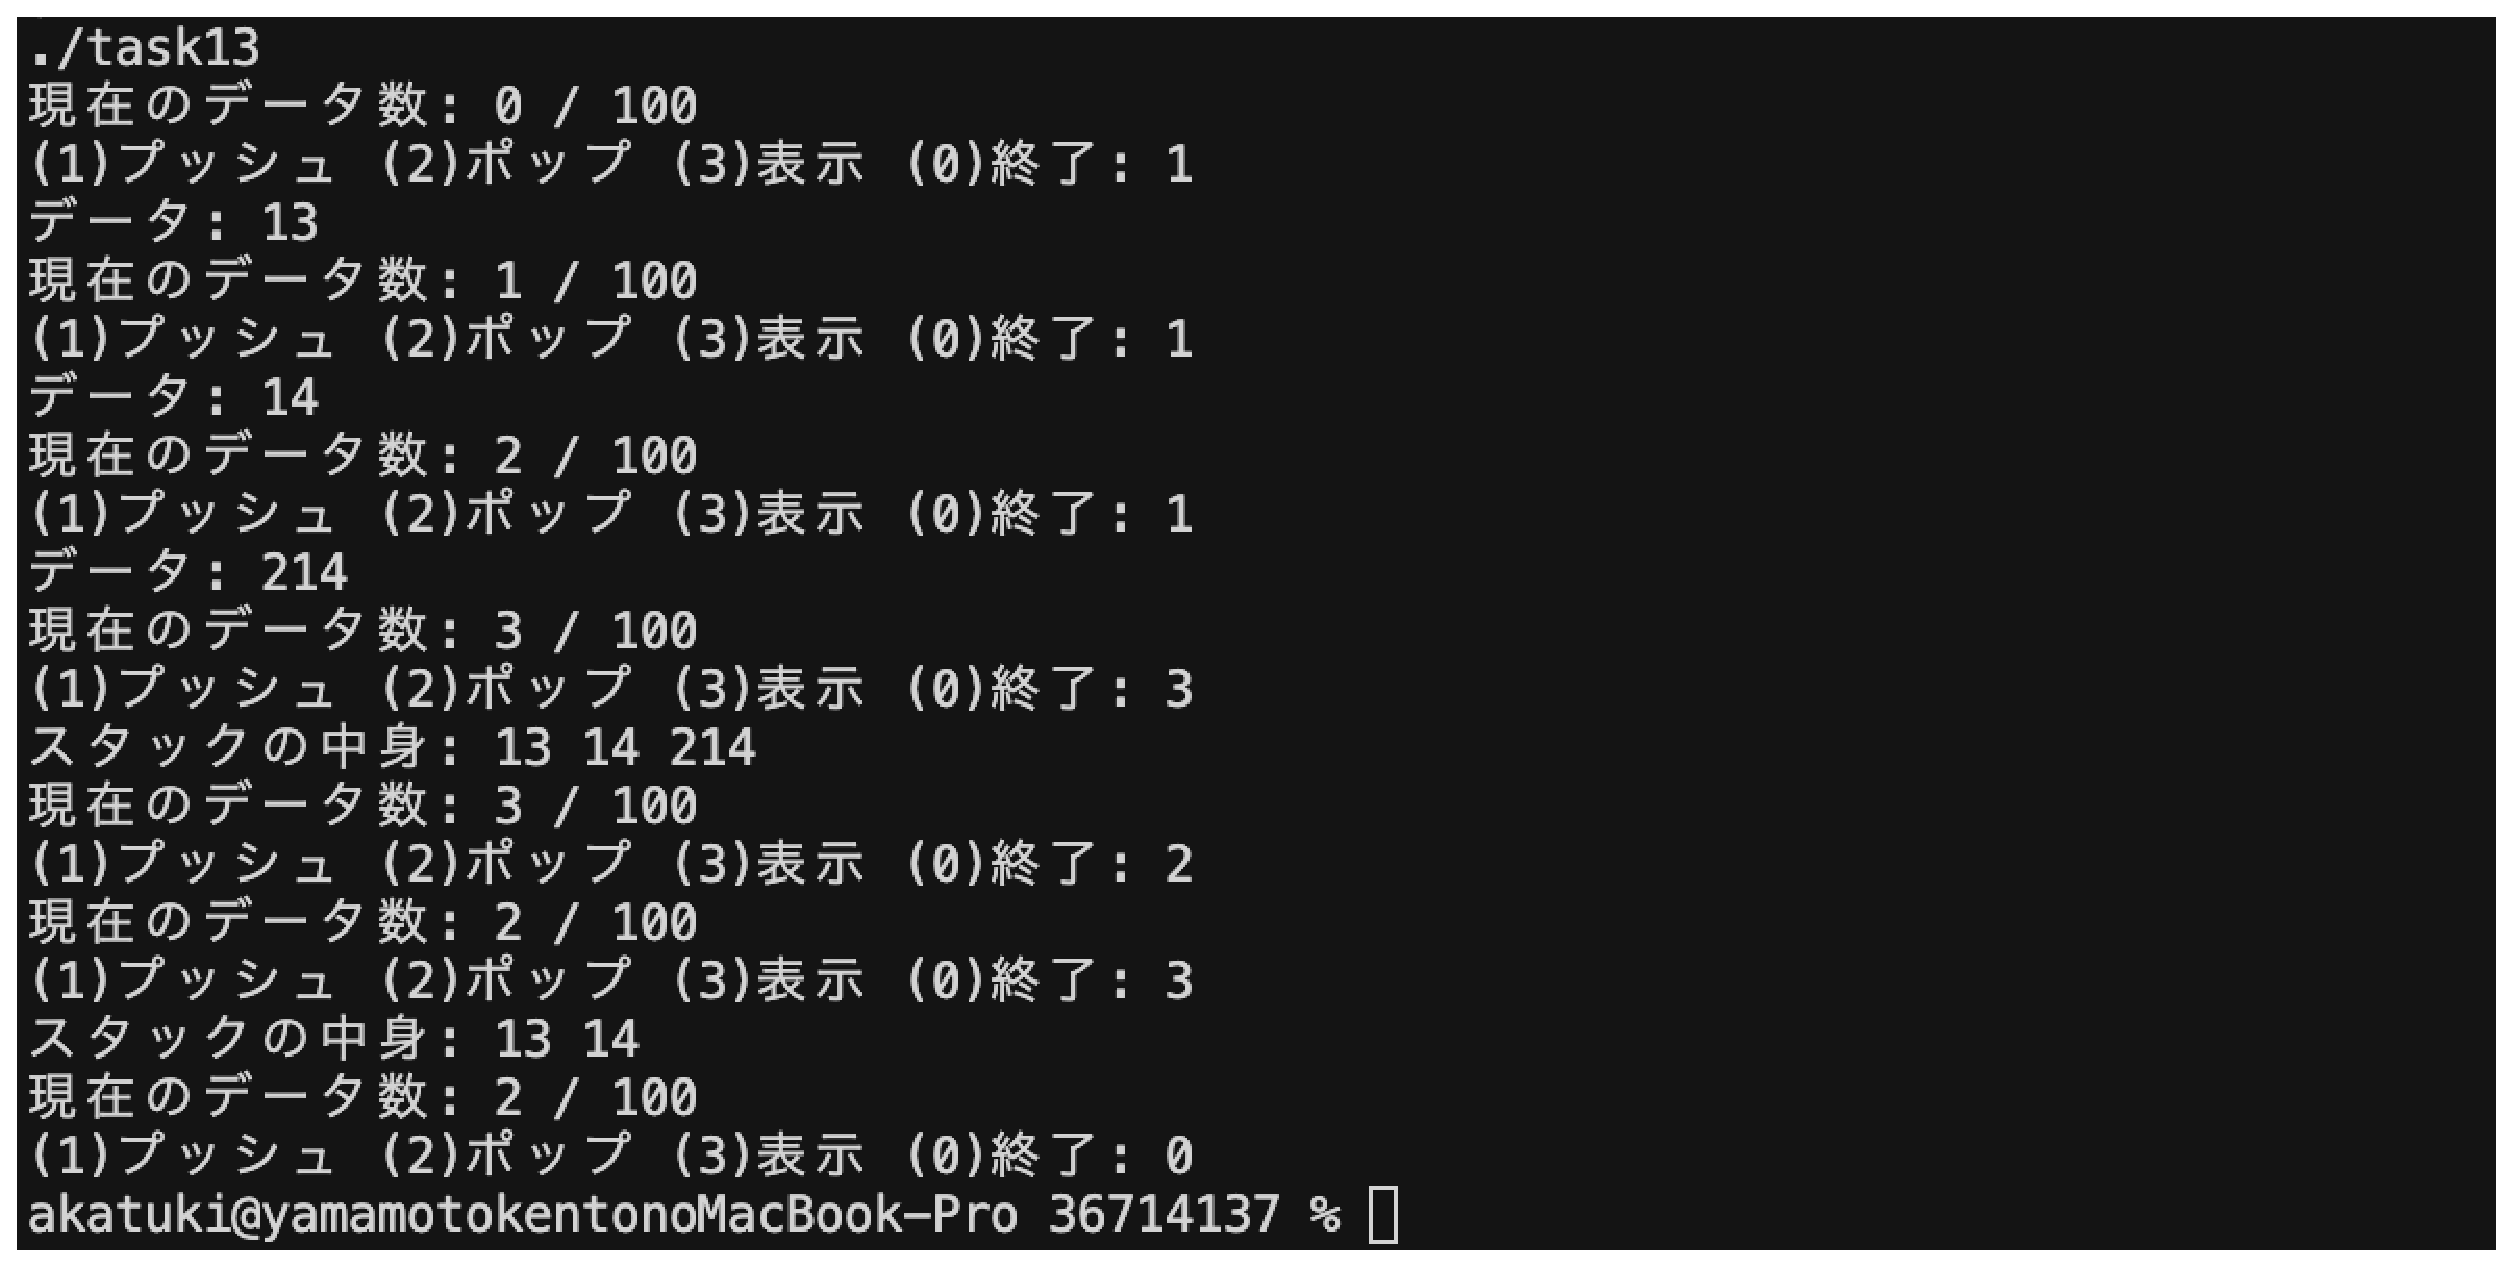
\includegraphics[width=0.8\textwidth]{images/13.eps}
  \caption{演習13-1の実行結果}
  \label{fig:task13}
\end{figure}

プッシュ、ポップ、全表示の各機能が正しく動作していることが確認できる。

\end{document}
